\chapter{Clasificación con descriptor LBP}
En este apartado se describirá la clase \textit{LBP}, dicha clase implementa el funcionamiento del descriptor LBP. También se describirá el proceso necesario para obtener la matriz de descriptores generados con LBP. Por último se mostrarán los resultados obtenidos por diferentes modelos y se comentarán y compararán con los obtenidos con el descriptor HOG. La implementación del descriptor, el archivo pruebas se pueden encontrar en los ficheros \textbf{lbp.py} y \textbf{prueba\_lbp.py}; la función utilizada para cargar los datos en el fichero de pruebas y la función utilizada para computar el descriptor para cada una de las imágenes se pueden encontrar en el fichero \textbf{functions.py}

Si se desea ejecutar los ficheros de prueba para este descriptor o para los siguientes, se puede descargar un \textit{.zip} con los ficheros de clases y datos que los ficheros de pruebas cargan para hacer después las pruebas. El enlace es el siguiente: \url{https://drive.google.com/file/d/1fm0rdfdmWWLU8sjTXU59laeOh27URCDa/view?usp=sharing}

\section{Implementación del descriptor LBP}
Para la implementar el descriptor LBP se ha creado una clase, llamada \textit{LBP}. Dicha clase contiene el tamaño de la ventana, el número de vecinos a comparar y el tamaño de bloque. Dentro de esta clase se encuentra la función \textit{computeLBPpixel()} dicha función se encarga de comparar el valor de cada píxel con sus vecinos y de computar el valor LBP con los resultados obtenidos de la comparación. También se encuentra la función \textit{computeLBPblock()}, dicha función toma como argumentos la posición inicial del bloque y la imagen y computa el valor de cada pixel dentro de los límites del bloque. Por último tenemos la función \textit{computeLBPWindows()}, que toma como argumento la posición del primer píxel de la ventana y la imagen, con estos datos va llamando a la función descrita anteriormente hasta computar la ventana entera. También está la función \textit{compute()} a la cual se le pasa la imagen y esta llama \textit{computeLBPWindow()}. \\

\begin{figure}[H]
	\centering
	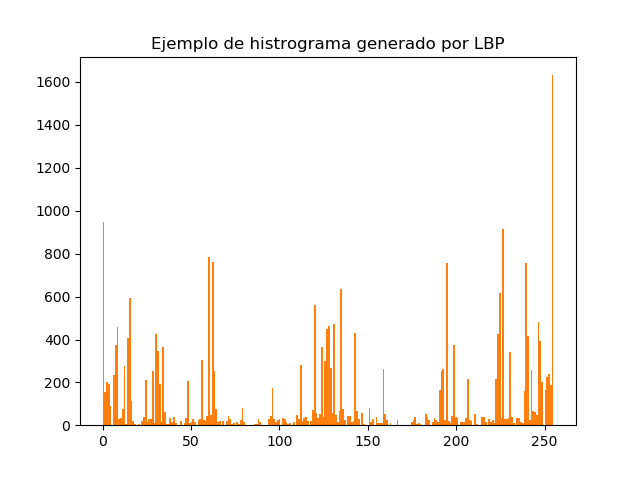
\includegraphics[width=140mm]{imagenes/lbp_histogram}
	\caption{Ejemplo Histograma de un descriptor LBP}
	\label{fig:salida_3}
\end{figure}

Una vez creada esta clase ya se pueden calcular los descriptores LBP para las imágenes. Para realizar la tarea de leer y computar los descriptores de la imágenes de forma general se ha implementado la función \textit{loadImages()} la cual toma de argumento un objeto de la clase del descriptor que se quiera utilizar siempre que su funcionamiento sea de la siguiente forma : descriptor.compute(imagen). Esta función se ha probado con HOG, la clase LBP implementada y la clase LBP-Uniforme, cuya descripción se encuentra en el siguiente apartado.

\section{Pruebas con LBP}
Para generar las validaciones con los diferentes modelos, se ha utilizado la función \textit{crossValidation()} (es la misma que se utiliza para el primer apartado) contenida en el archivo \textbf{functions.py}. Los resultados obtenidos son los siguientes:

\begin{table}[H]
	\begin{tabular}{llllll}
		\textbf{Validation} & \textbf{F1} & \textbf{accuracy} & \textbf{precision} & \textbf{truenegativerate} & \textbf{truepositiverate} \\
		0                   & 0.722057    & 0.740296          & 0.717092           & 0.751724                  & 0.727092                  \\
		1                   & 0.724521    & 0.747689          & 0.699805           & 0.745033                  & 0.751046                  \\
		2                   & 0.750000    & 0.767098          & 0.720000           & 0.754591                  & 0.782609                  \\
		3                   & 0.752753    & 0.771719          & 0.743083           & 0.779287                  & 0.762677                  \\
		4                   & 0.705385    & 0.742144          & 0.685832           & 0.754019                  & 0.726087                 
	\end{tabular}
	\caption{Validación con SVM kernel lineal}
	\label{table_10}
\end{table}

\begin{table}[H]
	\begin{tabular}{llllll}
		\textbf{Validation} & \textbf{F1} & \textbf{accuracy} & \textbf{precision} & \textbf{truenegativerate} & \textbf{truepositiverate} \\
		0                   & 0.609646    & 0.439002          & 0.438483           & 0.001645                  & 1.0                       \\
		1                   & 0.620778    & 0.450092          & 0.450092           & 0.000000                  & 1.0                       \\
		2                   & 0.612821    & 0.441774          & 0.441774           & 0.000000                  & 1.0                       \\
		3                   & 0.637681    & 0.468577          & 0.468085           & 0.001736                  & 1.0                       \\
		4                   & 0.611432    & 0.440850          & 0.440333           & 0.001650                  & 1.0                      
	\end{tabular}
	\caption{Validación con SVM kernel RBF}
	\label{table_11}
\end{table}

\begin{table}[H]
	\begin{tabular}{llllll}
		\textbf{Validation} & \textbf{F1} & \textbf{accuracy} & \textbf{precision} & \textbf{truenegativerate} & \textbf{truepositiverate} \\
		0                   & 0.757515    & 0.776340          & 0.744094           & 0.780405                  & 0.771429                  \\
		1                   & 0.742911    & 0.748614          & 0.711957           & 0.723958                  & 0.776680                  \\
		2                   & 0.752437    & 0.765250          & 0.735238           & 0.760757                  & 0.770459                  \\
		3                   & 0.738144    & 0.765250          & 0.720322           & 0.771757                  & 0.756871                  \\
		4                   & 0.754297    & 0.775416          & 0.732809           & 0.774086                  & 0.777083                 
	\end{tabular}
	\caption{Validación con SVM kernel polinómico grado 2}
	\label{table_12}
\end{table}

\begin{table}[H]
	\begin{tabular}{llllll}
		\textbf{Validation} & \textbf{F1} & \textbf{accuracy} & \textbf{precision} & \textbf{truenegativerate} & \textbf{truepositiverate} \\
		0                   & 0.762548    & 0.772643          & 0.745283           & 0.765625                  & 0.780632                  \\
		1                   & 0.769691    & 0.786506          & 0.745174           & 0.778894                  & 0.795876                  \\
		2                   & 0.753651    & 0.766174          & 0.706204           & 0.733002                  & 0.807933                  \\
		3                   & 0.763674    & 0.788355          & 0.728346           & 0.777778                  & 0.802603                  \\
		4                   & 0.768145    & 0.787431          & 0.750000           & 0.787625                  & 0.787190                 
	\end{tabular}
	\caption{Validación con SVM kernel polinómico grado 3}
	\label{table_13}
\end{table}

\begin{table}[H]
	\begin{tabular}{llllll}
		\textbf{Validation} & \textbf{F1} & \textbf{accuracy} & \textbf{precision} & \textbf{truenegativerate} & \textbf{truepositiverate} \\
		0                   & 0.347555    & 0.420518          & 0.352321           & 0.484034                  & 0.342916                  \\
		1                   & 0.359743    & 0.447320          & 0.365217           & 0.519737                  & 0.354430                  \\
		2                   & 0.288248    & 0.406654          & 0.311005           & 0.518395                  & 0.268595                  \\
		3                   & 0.727823    & 0.750462          & 0.691571           & 0.736928                  & 0.768085                  \\
		4                   & 0.373253    & 0.419593          & 0.349533           & 0.434146                  & 0.400428                 
	\end{tabular}
	\caption{Validación con SVM kernel polinómico grado 4}
	\label{table_14}
\end{table}

\begin{table}[H]
	\begin{tabular}{llllll}
		\textbf{Validation} & \textbf{F1} & \textbf{accuracy} & \textbf{precision} & \textbf{truenegativerate} & \textbf{truepositiverate} \\
		0                   & 0.613709    & 0.442699          & 0.442699           & 0.0                       & 1.0                       \\
		1                   & 0.612821    & 0.441774          & 0.441774           & 0.0                       & 1.0                       \\
		2                   & 0.624285    & 0.453789          & 0.453789           & 0.0                       & 1.0                       \\
		3                   & 0.623410    & 0.452865          & 0.452865           & 0.0                       & 1.0                       \\
		4                   & 0.624285    & 0.453789          & 0.453789           & 0.0                       & 1.0                      
	\end{tabular}
	\caption{Validación con SVM kernel polinómico grado 5}
	\label{table_15}
\end{table}

\begin{table}[H]
	\begin{tabular}{llllll}
		\textbf{Validation} & \textbf{F1} & \textbf{accuracy} & \textbf{precision} & \textbf{truenegativerate} & \textbf{truepositiverate} \\
		0                   & 0.619898    & 0.449168          & 0.449168           & 0.0                       & 1.0                       \\
		1                   & 0.626032    & 0.455638          & 0.455638           & 0.0                       & 1.0                       \\
		2                   & 0.609254    & 0.438078          & 0.438078           & 0.0                       & 1.0                       \\
		3                   & 0.607465    & 0.436229          & 0.436229           & 0.0                       & 1.0                       \\
		4                   & 0.629512    & 0.459335          & 0.459335           & 0.0                       & 1.0                      
	\end{tabular}
	\caption{Validación con SVM kernel sigmoidal}
	\label{table_16}
\end{table}

\begin{table}[H]
	\begin{tabular}{llllll}
		\textbf{Validation} & \textbf{F1} & \textbf{accuracy} & \textbf{precision} & \textbf{truenegativerate} & \textbf{truepositiverate} \\
		0                   & 0.619017    & 0.448244          & 0.448244           & 0.000000                  & 1.0                       \\
		1                   & 0.626429    & 0.456562          & 0.456059           & 0.001698                  & 1.0                       \\
		2                   & 0.625478    & 0.456562          & 0.455051           & 0.005076                  & 1.0                       \\
		3                   & 0.612323    & 0.441774          & 0.441258           & 0.001653                  & 1.0                       \\
		4                   & 0.609646    & 0.439002          & 0.438483           & 0.001645                  & 1.0                      
	\end{tabular}
	\caption{Validación con SVM kernel Chi Cuadrado}
	\label{table_17}
\end{table}

\begin{table}[H]
	\begin{tabular}{llllll}
		\textbf{Validation} & \textbf{F1} & \textbf{accuracy} & \textbf{precision} & \textbf{truenegativerate} & \textbf{truepositiverate} \\
		0                   & 0.922912    & 0.933457          & 0.907368           & 0.929374                  & 0.938998                  \\
		1                   & 0.926625    & 0.935305          & 0.920833           & 0.937500                  & 0.932489                  \\
		2                   & 0.924731    & 0.935305          & 0.932755           & 0.949429                  & 0.916844                  \\
		3                   & 0.934322    & 0.942699          & 0.928421           & 0.944535                  & 0.940299                  \\
		4                   & 0.939516    & 0.944547          & 0.939516           & 0.948805                  & 0.939516                 
	\end{tabular}
	\caption{Validación con SVM kernel Inter}
	\label{table_18}
\end{table}

Como se puede ver, alguno de los resultados obtenidos rondan entre el 70-75\%, por ejemplo el clasificador con kernel lineal, o algunos de los kernels polinómico de grado bajo. Otros clasificadores obtiene resultados muy pobres, sobreajustándose a los datos y prediciendo todos los valores a uno, eso pasa en los clasificadores polinómicos de grado mayor, el clasificador de kernel RBF, el clasificador de kernel sigmoidal y el clasificador de kernel Chi Cuadrado. En cambio, el clasificador con kernel Inter obtiene resultados en todas sus validaciones algo mayores del 90\% y es con diferencia el mejor clasificador encontrado para LBP. \\

A excepción del clasificador con kernel Inter, que obtiene resultados muy parejos tanto con descriptores HOG como con descriptores LBP, los resultados obtenidos por los clasificadores entrenados con descriptores LBP son peores que los obtenidos por HOG. Esto puede ser por la diferencia en el número de características que se obtienen de cada uno, para el caso de HOG se extraen 3780 características por imagen y para LBP 26880, la gran características de este último puede provocar que los clasificadores obtenidos sufran de sobreaprendizaje. Además, uno de los problemas de LBP es que contiene valores entre 0 y 255, de los cuales solamente unos pocos son realmente relevantes (existen formas de evitar este problema como se verá en el siguiente caso ), esto puede estar provocando también este peor rendimiento de los clasificadores.
